% External PNG figures; native PGFPlots graphs read ordinary CSV files.
\documentclass[10pt,a4paper]{article}
\usepackage[margin=18mm,headheight=14pt,headsep=7mm,footskip=10mm]{geometry}
\usepackage[T1]{fontenc}\usepackage[utf8]{inputenc}
\usepackage{lmodern,amsmath,graphicx,booktabs,array,caption,xcolor,fancyhdr,hyperref,pgfplots}
\pgfplotsset{compat=1.18}
\definecolor{Navy}{HTML}{17354B}\definecolor{Teal}{HTML}{166979}
\hypersetup{colorlinks=true,urlcolor=Teal,linkcolor=Teal,pdftitle={Power board: edge-battery lateral pull},pdfauthor={MIT Rocket Team -- simulation study}}
\captionsetup{font=small,labelfont=bf,justification=raggedright,singlelinecheck=false,hypcap=false}
\pagestyle{fancy}\fancyhf{}
\fancyhead[L]{\small\color{Navy}MIT Rocket Team \enspace | \enspace Power board}
\fancyhead[R]{\small\color{Navy}Battery lateral pull}
\fancyfoot[L]{\footnotesize Report issued 5 October 2026}\fancyfoot[R]{\footnotesize\thepage}
\renewcommand{\headrulewidth}{0.3pt}
\setlength{\parindent}{0pt}\setlength{\parskip}{5pt}\setlength{\emergencystretch}{2em}
\renewcommand{\arraystretch}{1.1}
\newcommand{\ReportHeading}[1]{\par\vspace{7pt}{\large\bfseries\color{Teal}#1}\par\vspace{3pt}}
\newcommand{\PageTitle}[1]{{\LARGE\bfseries\color{Navy}#1\par}\vspace{7pt}}
\begin{document}
\PageTitle{Power board: edge-battery lateral pull}
{\large\color{Teal}Exploratory yielding, clamp contact and deformation study}\par
{\small ANSYS MAPDL 2026 R1.02 \enspace | \enspace Quasistatic, large deformation}\par
The question is how much sideways load an edge battery can carry before its nickel strip tears near a washer. This study reconstructs the two nickel attachments of one edge battery and calculates their nonlinear response to lateral displacement. It provides a load--displacement baseline and identifies the limits of a numerical tearing prediction.

\textbf{A defensible breaking force has not been established.} The model includes plasticity and, in the contact cases, washer friction. It contains no calibrated fracture or weld-failure law; therefore it cannot simulate a physical snap. The reported forces are demands at a prescribed displacement, not allowable loads or ultimate strengths.

\ReportHeading{Principal finding}
For the ideal fixed-clamp model with an illustrative annealed-nickel yield stress of 148 MPa, the refined mesh gives \textbf{8.21 N at 0.50 mm} battery-centre displacement. The battery rotates by approximately \textbf{2.70 degrees} about Y. The coarse result is 8.63 N. The response is dominated by local bending of the thin attachment strips.

Peak equivalent plastic strain from the shell element summaries rises from \textbf{1.34\% to 2.46\%} under mesh refinement. This strong local sensitivity prevents a strain-based failure claim. The force at the endpoint changes by 5.18\% relative to the fine result.

\begin{center}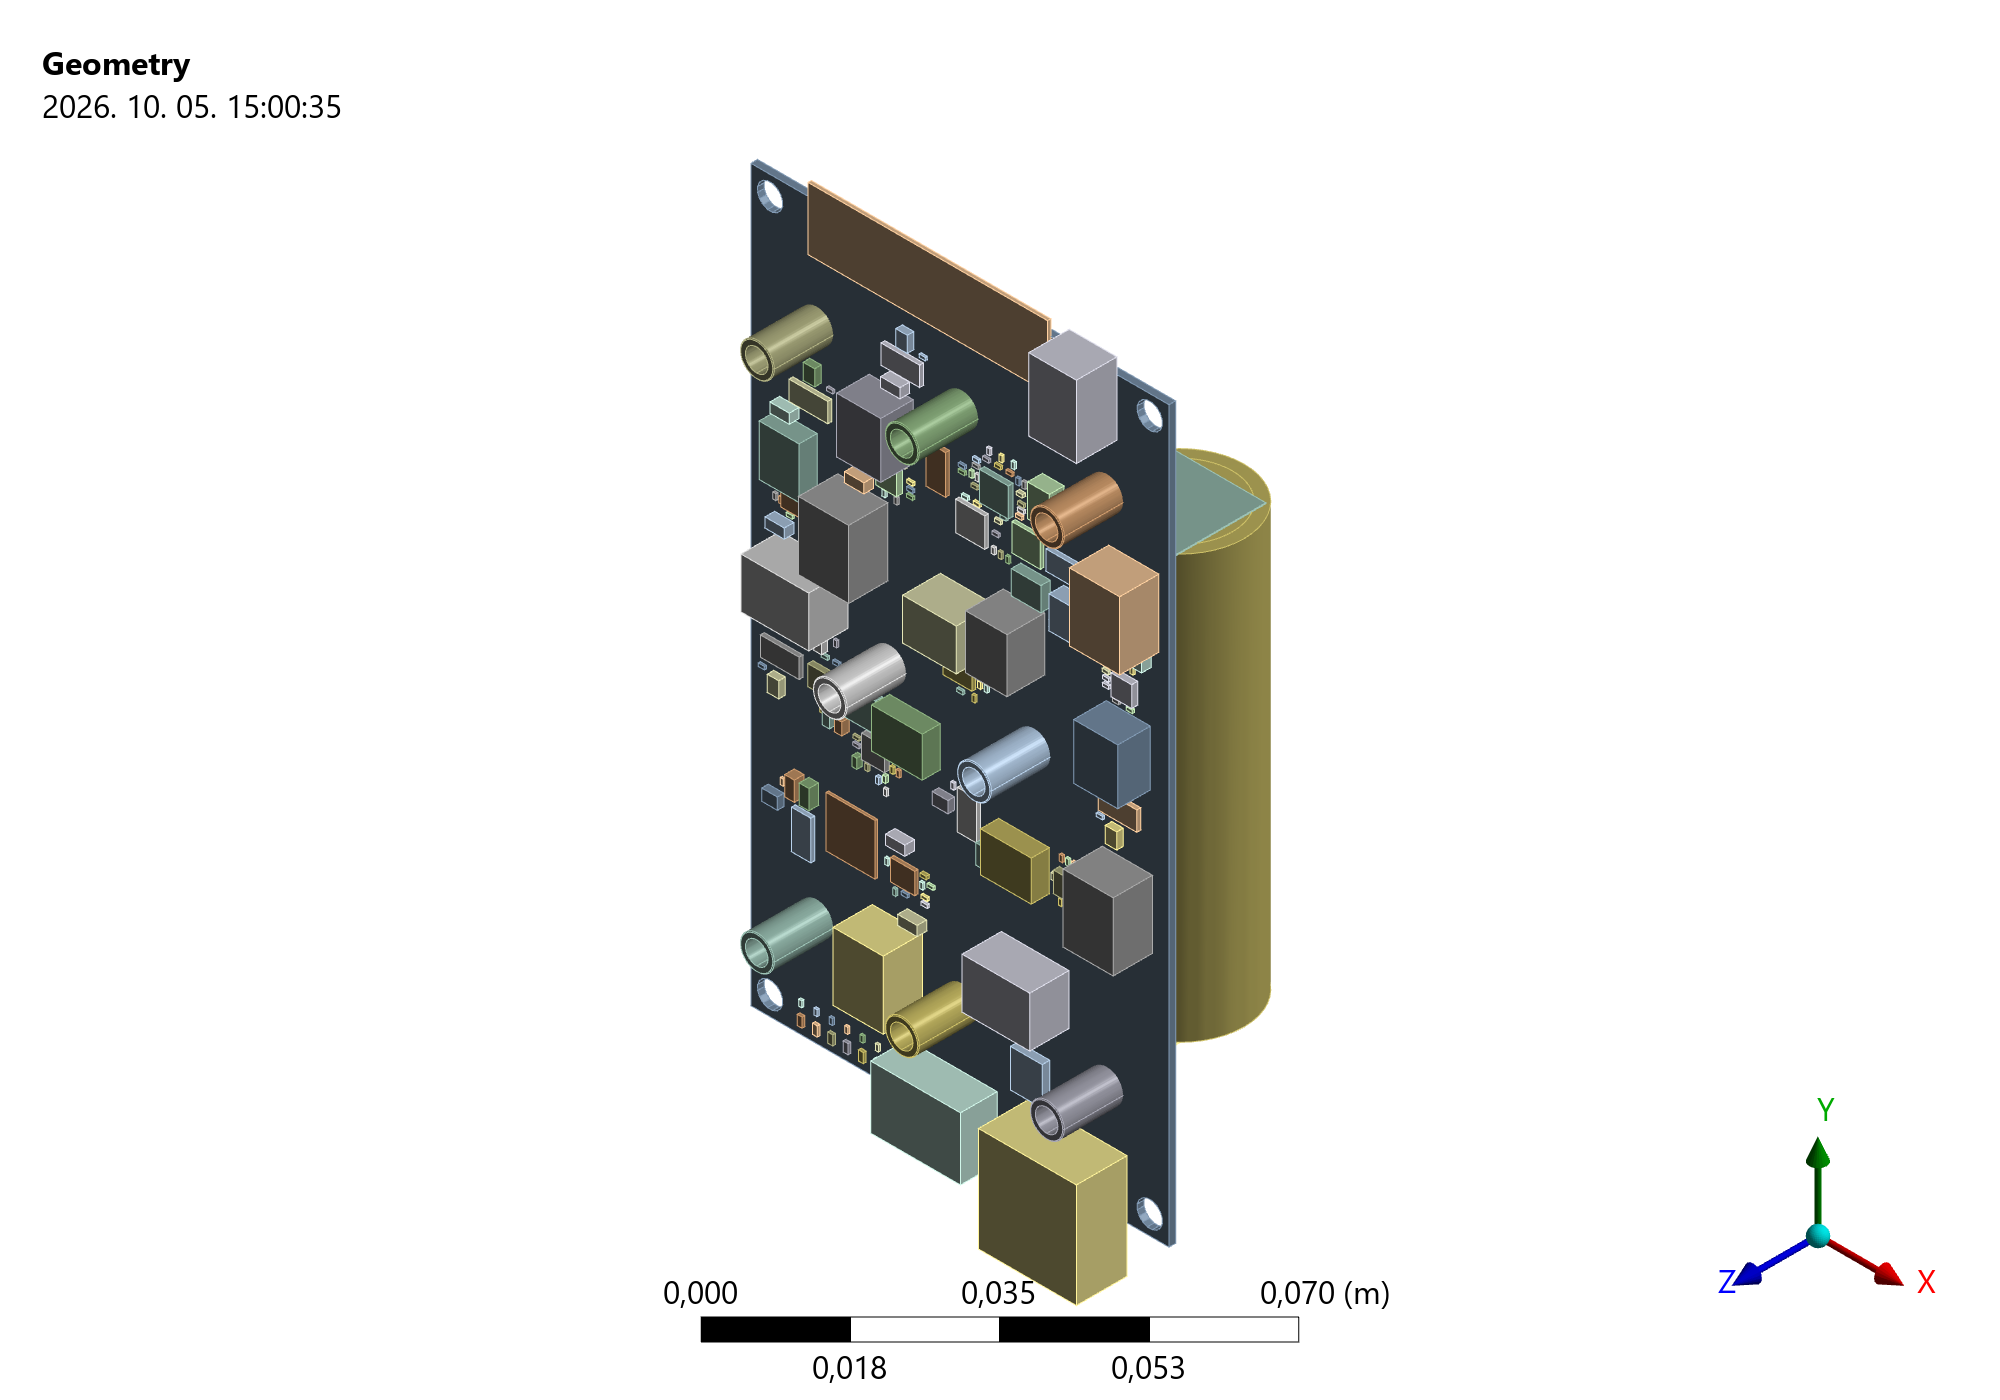
\includegraphics[width=.78\linewidth,height=78mm,keepaspectratio]{figures/assembly_geometry.png}
\captionof{figure}{Original populated power-board geometry, for assembly context. This new calculation solves a local attachment model; it does not solve the full PCB or all components. The previous modal and random-vibration studies remain separate.}\end{center}
\textbf{With 750 N initially applied at each of the two modeled washers}, the refined frictional-contact model requires 8.12 N at 0.50 mm. This is a deformation demand under the stated assumptions, not a rupture load.

\ReportHeading{What this answers}
The calculation establishes where plastic deformation concentrates, the reaction needed for a specified battery movement, and sensitivity to mesh and assumed nickel strength. Predicting the load at actual tearing requires measured strip plasticity, fracture calibration and a validated representation of the washer, weld and supporting board.

\clearpage\PageTitle{Geometry and load path}
\begin{center}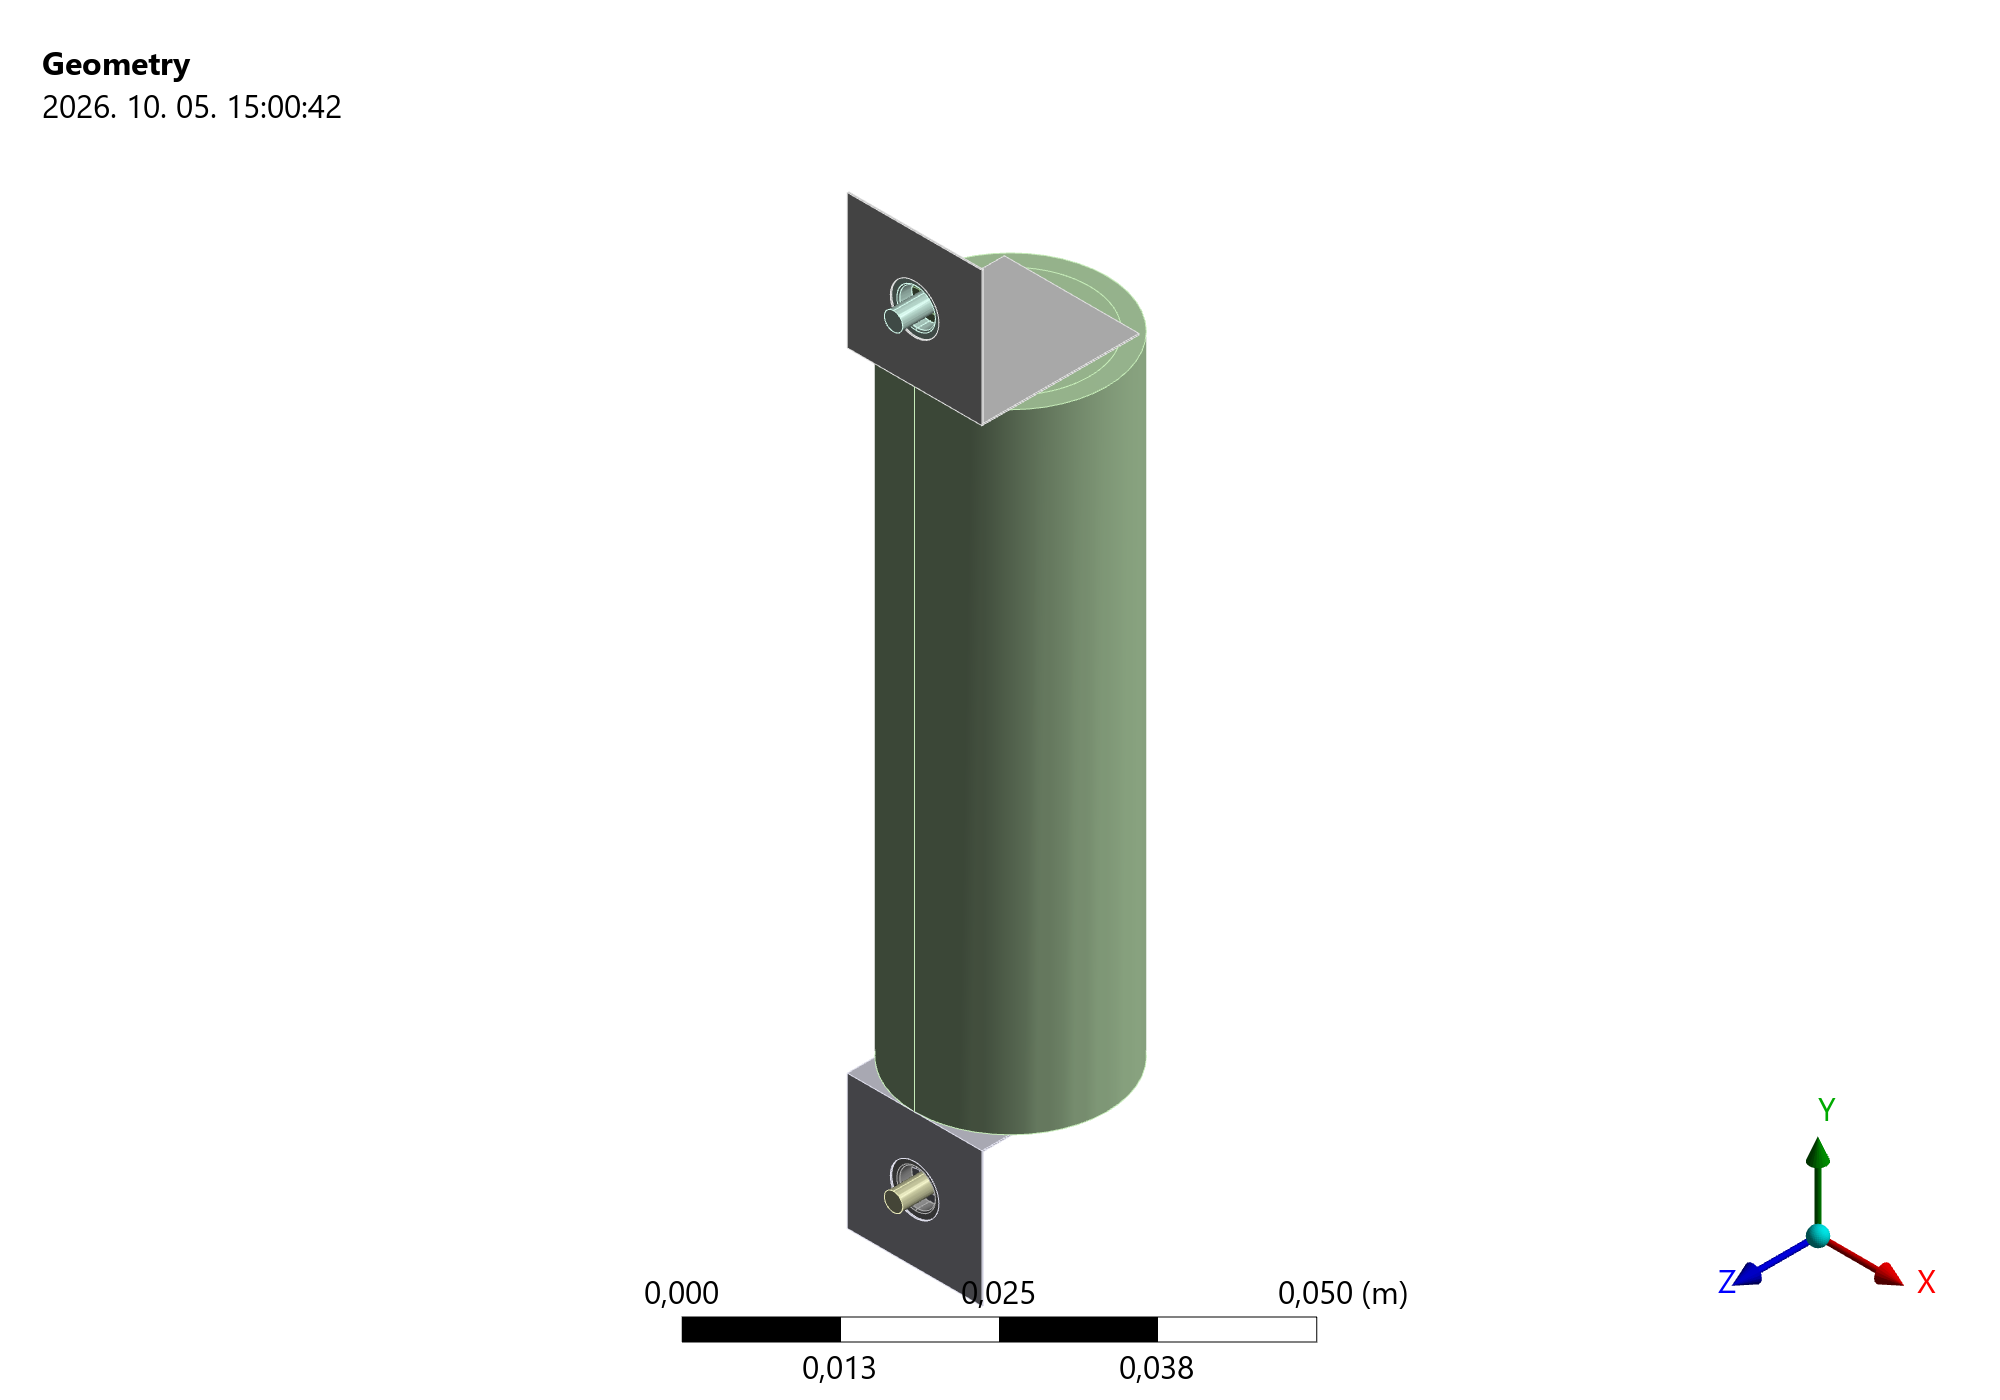
\includegraphics[width=.78\linewidth,height=72mm,keepaspectratio]{figures/edge_battery_cad.png}
\captionof{figure}{Selected edge battery and its two nickel strips and fasteners from the source CAD. Geometry IDs: battery 20157 (Part 27[1]); strips 20091 and 20348; washers 20246 and 20466.}\end{center}
\begin{center}\begin{tabular}{p{.47\linewidth}p{.43\linewidth}}\toprule
\textbf{Quantity} & \textbf{CAD-derived value}\\\midrule
Strip thickness; width & 0.15 mm; 15.0 mm\\
Flat leg; vertical leg & Approximately 15.0 mm; 17.5 mm\\
Strip hole diameter & 5.408 mm\\
Washer outer diameter & 11.1252 mm\\
Battery radius; end-face separation & 10.7 mm; 70.0 mm\\
Battery reference point $(x,y,z)$ & $(10.803671,60.407,-11.822674)$ mm\\
Washer-centre Y coordinates & 17.906999 and 102.907004 mm\\\bottomrule
\end{tabular}\end{center}
Thickness was obtained from paired planar face centroids; hole radius from cylindrical face area divided by $\pi t$. A midsurface shell reconstruction shifts the bend intersection by half the thickness. Sharp bend lines replace the detailed formed radius; fillets are omitted.

\ReportHeading{Boundary conditions}
The battery is rigid, represented by a central reference node and rigid links to the portions of both vertical strips lying within the battery-end circular footprint. This assumes a perfect, broad nickel-to-battery attachment; an actual spot-weld pattern is not known. Displacement control tracks the post-yield path, and the required force is read from its reaction. Only battery-centre UX is prescribed during the sideways pull. UY, UZ and all three rotations are free. Separate cases use $+X$ and $-X$; both ramp to $|u_X|=0.5$ mm. This endpoint is an exploratory displacement limit chosen to observe the initial plastic mechanism. It is not a measured failure displacement or the maximum load the joint can carry.

There is \textbf{no battery-to-PCB connection or contact}. The PCB, its other components, the two other batteries and the other four bolts are excluded from this local calculation. Fixed clamp supports replace PCB compliance. These assumptions permit battery rotation and must match the intended physical test fixture.

\ReportHeading{Seating assumption requiring confirmation}
The imported geometry contains about 0.5715 mm clearance between the nickel top surface and PCB underside, and about 0.0245 mm between washer and nickel. The local model assumes a fully seated strip between the washer and its backing support. It does not simulate closure of these CAD gaps or stand-off bending. Verify the real stack-up before interpreting the calculated force as assembly performance.

\clearpage\PageTitle{Nickel model and data provenance}
The user specified 99.6\% nickel. Commercially pure Nickel 200 is used as a substitute data source, not as a certified identification of the actual strip. Purity alone does not establish temper, yield strength, work hardening or fracture strain.

\begin{center}\begin{tabular}{p{.25\linewidth}p{.29\linewidth}p{.35\linewidth}}\toprule
\textbf{Input} & \textbf{Value used} & \textbf{Basis}\\\midrule
Young's modulus & 205 GPa & Nickel 200 bulletin, Table 4, 26\,$^\circ$C [1]\\
Poisson ratio & 0.29 & Same source [1]\\
Baseline yield stress & 148 MPa & Typical annealed Nickel 200 handbook value [2]\\
Yield sensitivity & 105 and 210 MPa & Ends of published annealed-strip range [1]\\
Bilinear tangent $E_t$ & 1,000 MPa & Exploratory assumption; no measured curve\\
Clamp friction coefficient & 0.20 & Exploratory assumption; no joint test\\
Preload & 750 N per modeled washer & User specification; two modeled washers\\
Fracture / damage data & None & No damage evolution or element deletion\\\bottomrule
\end{tabular}\end{center}
The manufacturer's annealed-strip range is 105--210 MPa yield stress and 380--520 MPa ultimate tensile strength, with 40--55\% elongation over a 51 mm gauge length [1]. The same bulletin gives much higher strengths for spring-temper strip. Consequently, the annealed range is a conditional sensitivity study, not a proven bound for this hardware.

\ReportHeading{Constitutive law}
An isotropic, rate-independent von Mises bilinear plasticity law is used through \texttt{TB,BISO}. The 1 GPa value is the post-yield slope in total uniaxial strain. Its equivalent slope with respect to plastic strain is
\[
H=\frac{E E_t}{E-E_t}=1.0049\ \mathrm{GPa}.
\]
No temperature change, strain-rate dependence, residual stress from forming, fatigue, gravity or inertia is included. Material density is not needed for this static calculation. Damping is not relevant to the quasistatic analysis.

\ReportHeading{Why published elongation is not a fracture criterion}
Gauge-length elongation contains distributed plastic deformation and necking. It is not a transferable local equivalent-plastic-strain limit for the multiaxial washer-edge state. Similarly, reaching a handbook tensile strength at one stress concentration does not prove that the joint snaps. Neither quantity is used here to delete elements or declare failure.

For a calibrated prediction, measure the actual strip's true stress--plastic-strain curve and fracture response, including stress-state dependence. Resolve the washer-edge three-dimensional stress state and use a mesh-regularized damage law supported by joint tests [6]. Thin shell plasticity cannot resolve through-thickness washer indentation or a discrete tear.
\clearpage\PageTitle{Force, direction and material sensitivity}
\begin{center}\begin{tikzpicture}\begin{axis}[width=\linewidth,height=65mm,xlabel={Battery centre displacement magnitude (mm)},ylabel={Lateral reaction magnitude (N)},xmin=0,xmax=.5,grid=both,minor tick num=1,legend style={font=\footnotesize,at={(.98,.03)},anchor=south east,fill=white},tick label style={font=\small},xticklabel style={/pgf/number format/fixed,/pgf/number format/precision=2},label style={font=\small}]
\addplot+[color=Teal,thick,mark=none] table[col sep=comma,x=displacement_mm,y=force_N] {data/grip_lagrange_curve.csv};\addlegendentry{2,304 shells}
\addplot+[color=Navy,thick,mark=none] table[col sep=comma,x=displacement_mm,y=force_N] {data/grip_fine_lagrange_curve.csv};\addlegendentry{9,216 shells}
\end{axis}\end{tikzpicture}

\captionof{figure}{Ideal fixed-clamp response at two mesh densities. Lines connect converged saved substeps. Origin is the unloaded reference. Forces are magnitudes of the single battery reference-node reaction.}\end{center}
\begin{center}\begin{tikzpicture}\begin{axis}[width=\linewidth,height=65mm,xlabel={Battery centre displacement magnitude (mm)},ylabel={Lateral reaction magnitude (N)},xmin=0,xmax=.5,grid=both,minor tick num=1,legend style={font=\footnotesize,at={(.98,.03)},anchor=south east,fill=white},tick label style={font=\small},xticklabel style={/pgf/number format/fixed,/pgf/number format/precision=2},label style={font=\small}]
\addplot+[color=Teal,thick,mark=none] table[col sep=comma,x=displacement_mm,y=force_N] {data/grip_soft_lagrange_curve.csv};\addlegendentry{Yield 105 MPa}
\addplot+[color=Navy,thick,mark=none] table[col sep=comma,x=displacement_mm,y=force_N] {data/grip_lagrange_curve.csv};\addlegendentry{Yield 148 MPa}
\addplot+[color=orange!85!black,thick,mark=none] table[col sep=comma,x=displacement_mm,y=force_N] {data/grip_strong_lagrange_curve.csv};\addlegendentry{Yield 210 MPa}
\end{axis}\end{tikzpicture}

\captionof{figure}{Conditional annealed-yield sensitivity on the 2,304-shell mesh. Elastic constants and the assumed post-yield tangent are unchanged.}\end{center}
\begin{center}\begin{tabular}{l r r r}\toprule
\textbf{Fixed-clamp case} & \textbf{$|F_X|$ at 0.5 mm (N)} & \textbf{$\bar\varepsilon^p_\mathrm{max}$ (\%)} & \textbf{Shells}\\\midrule
Baseline, +X & 8.633 & 1.344 & 2,304 \\
Refined, +X & 8.207 & 2.464 & 9,216 \\
Baseline, -X & 8.597 & 1.342 & 2,304 \\
Yield 105 MPa, +X & 6.346 & 1.370 & 2,304 \\
Yield 210 MPa, +X & 11.762 & 1.301 & 2,304 \\
\bottomrule\end{tabular}\end{center}
The baseline $+X$ and $-X$ endpoint reactions differ by approximately 0.42\%. Small differences reflect the slight geometric offset and nonlinear response. The tabulated plastic strain is the largest top/bottom shell \emph{element-summary} value, not a resolved integration-point fracture strain. First detected plasticity depends on saved-substep spacing; it is not reported as an exact yield force.

\clearpage\PageTitle{Deformation and plastic concentration}
\begin{center}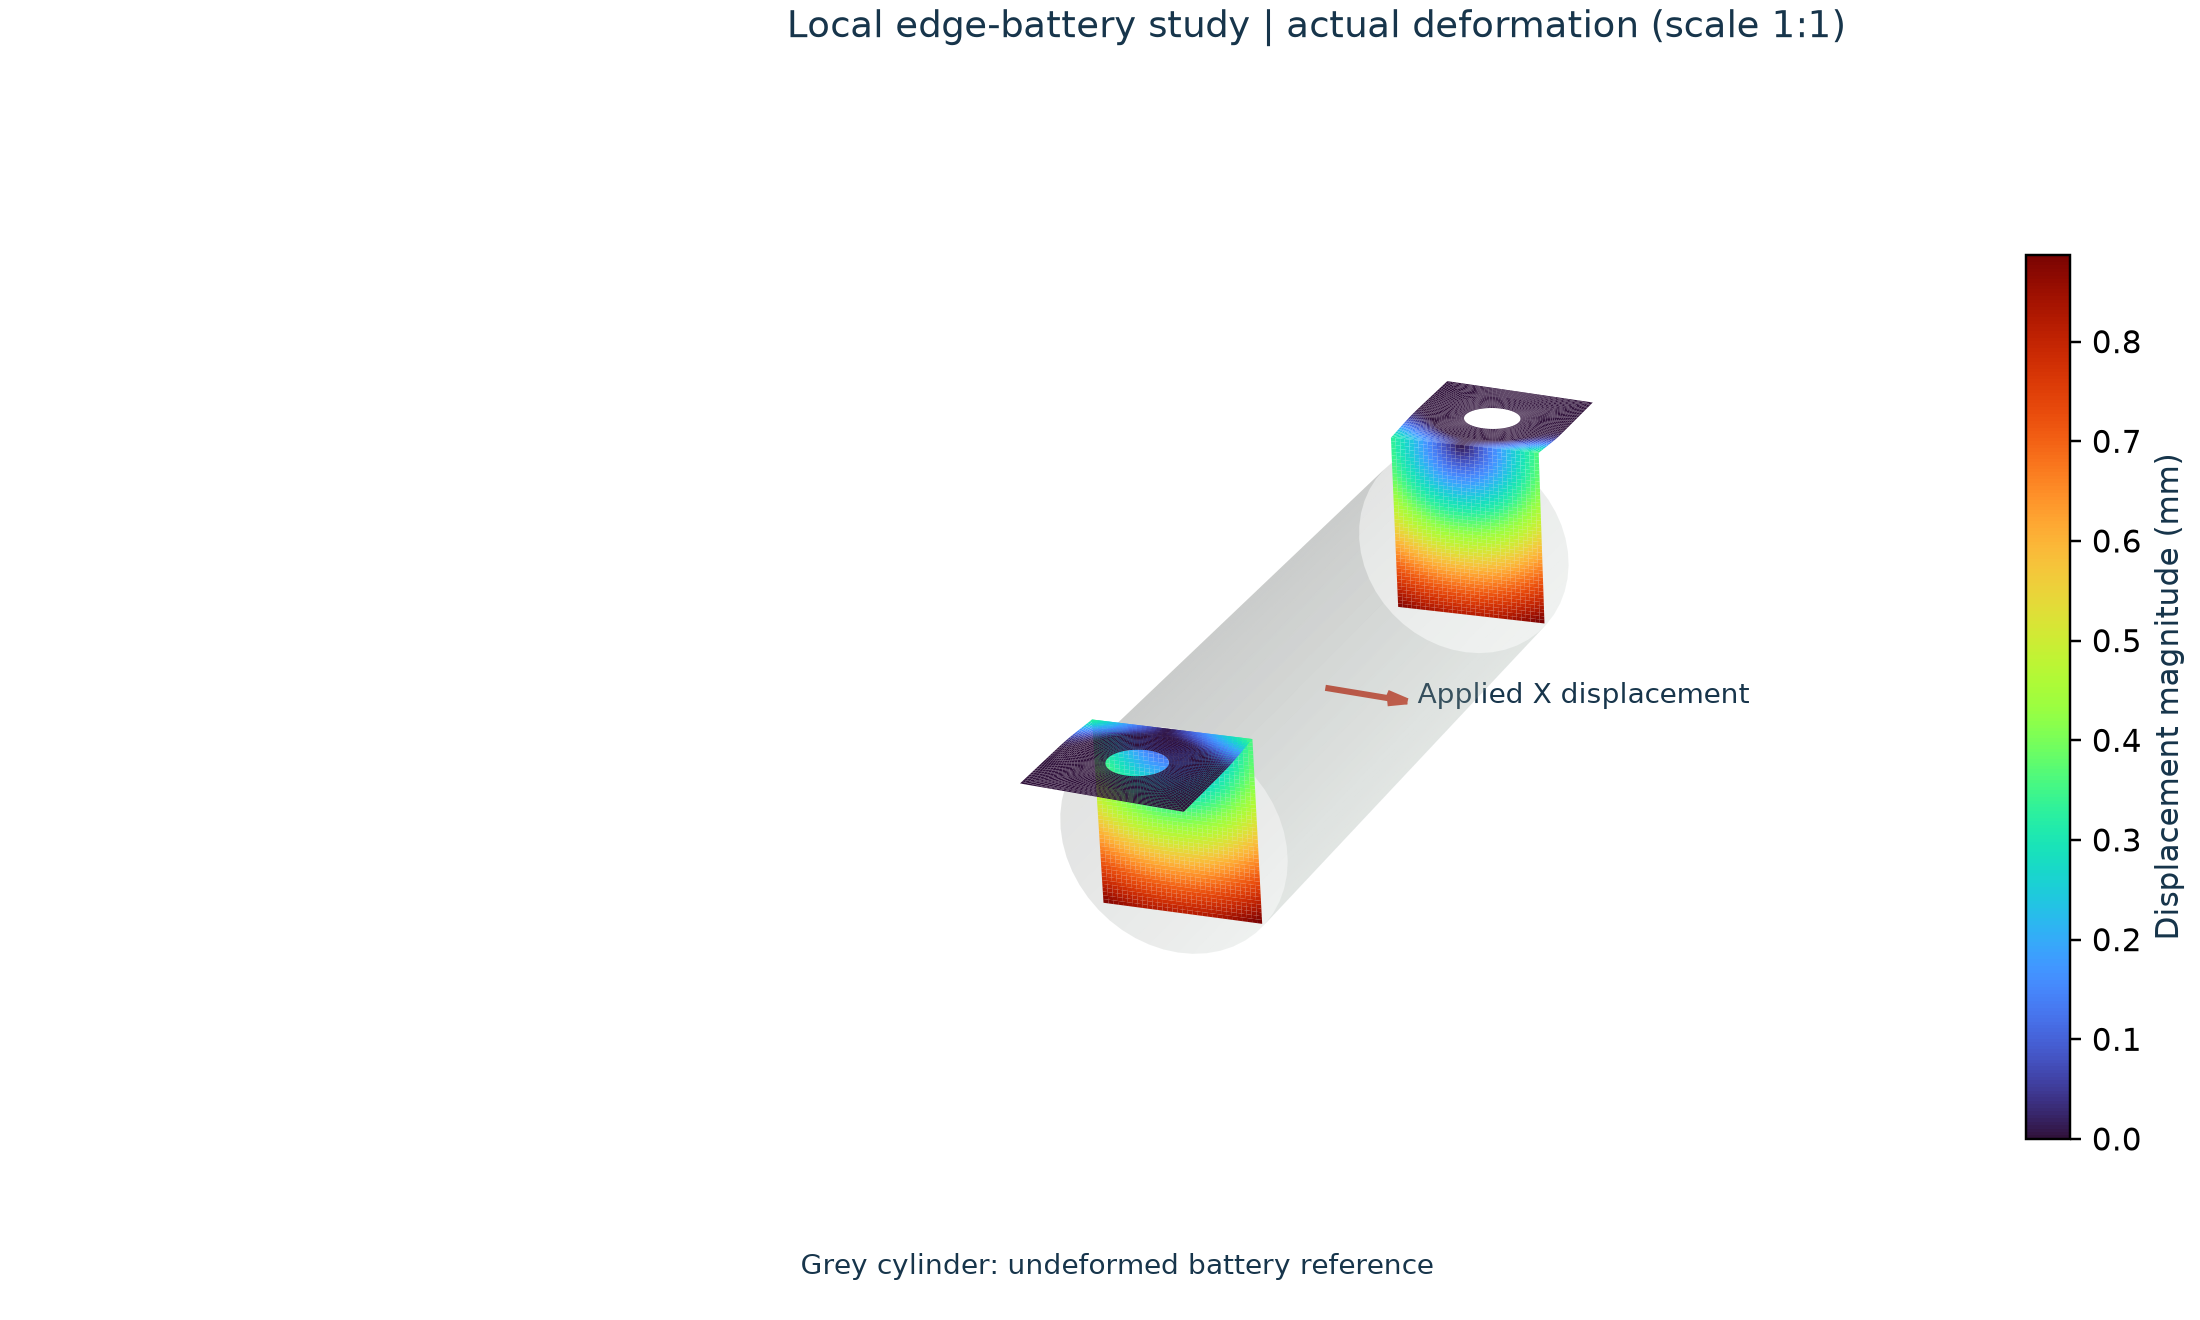
\includegraphics[width=.89\linewidth,height=99mm,keepaspectratio]{figures/grip_fine_lagrange_deformation.png}
\captionof{figure}{Refined ideal-clamp model at $u_X=+0.5$ mm; deformation scale 1:1. Colour is the shell displacement magnitude, averaged over each plotted element. The grey cylinder is an undeformed geometric battery reference, not a solved flexible battery contour. Strip points can move more than 0.5 mm because the battery also rotates.}\end{center}
\begin{center}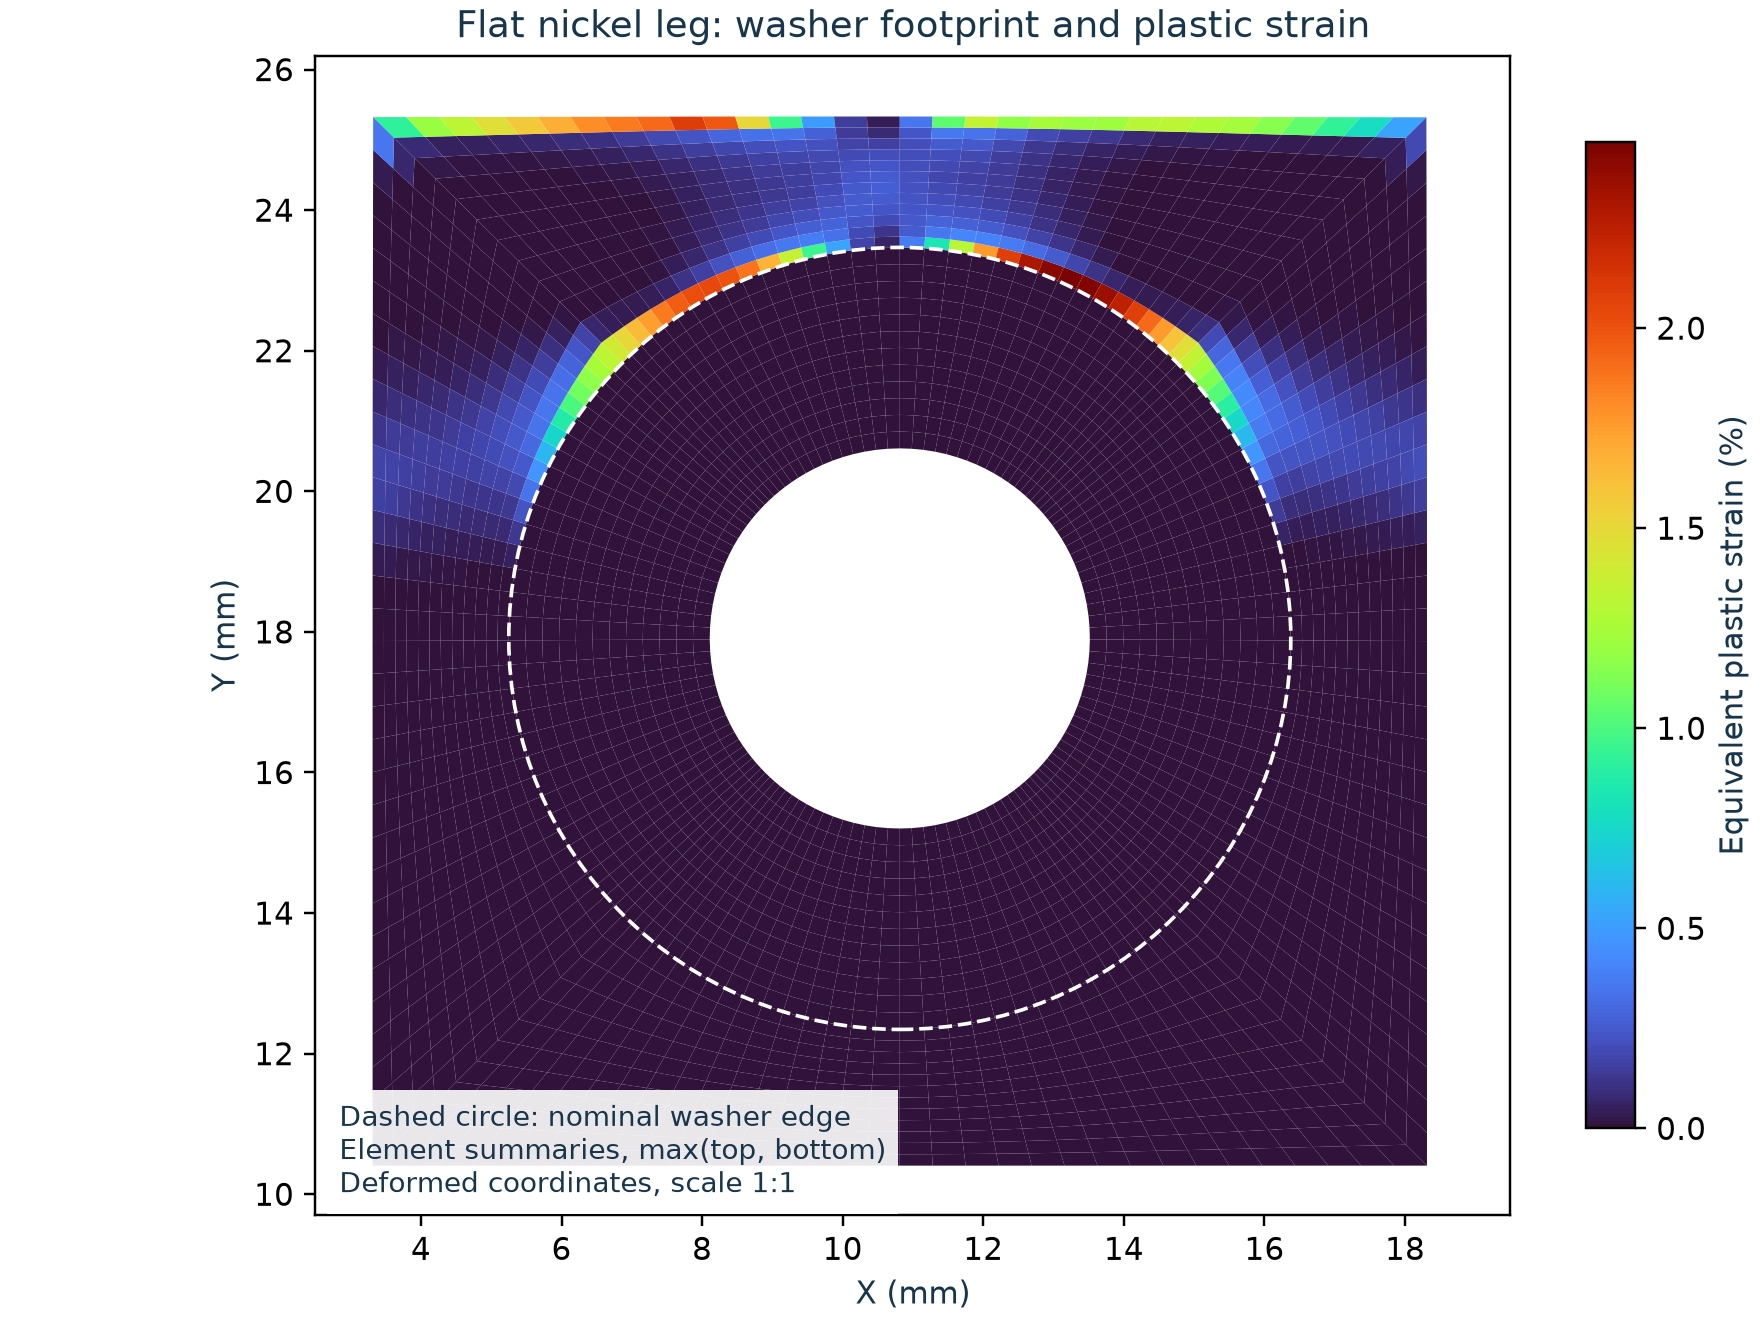
\includegraphics[width=.71\linewidth,height=90mm,keepaspectratio]{figures/grip_fine_lagrange_plastic_plan.png}
\captionof{figure}{Plastic strain on the lower flat nickel leg of the refined fixed-clamp model. Dashed circle marks the nominal washer outer edge. Values are the larger of top/bottom element summaries; deformation is shown at scale 1:1.}\end{center}
Plasticity concentrates near the imposed washer-edge restraint and adjoining free strip. The ideal fixed clamp and sharp geometric transitions accentuate this local concentration. The 83.4\% increase in peak plastic strain upon refinement shows why this field cannot yet be used to infer a tearing force.
\clearpage\PageTitle{750 N washer contact cases}
Two rigid annular platens sandwich each strip over the washer footprint. Frictional CONTA174/TARGE170 pairs permit tangential slip and separation, with an assumed Coulomb coefficient of 0.20. The bolt shafts, threads and PCB are not modeled explicitly.

In load step 1, 750 N is applied to each lower platen while the battery reference point is temporarily held. At the converged preload state, each lower platen's Z displacement is locked and its applied force is removed. Load step 2 transfers the force to displacement control with stepped loading while the battery remains held, preventing a spurious unloading ramp. In step 3, five battery reference DOFs are released and UX is ramped to $\pm0.5$ mm. The locked rigid platens are a stiff-clamp approximation, not a finite-stiffness bolt pretension model.

Contact uses an augmented-Lagrange formulation, shell-thickness offsets, normal stiffness factor 0.1, penetration tolerance factor 0.01 and 0.2 mm pinball radius. These are numerical settings, not measured material properties. Unsymmetric Newton iteration is used for the frictional cases [5].
\begin{center}\begin{tikzpicture}\begin{axis}[width=\linewidth,height=65mm,xlabel={Battery centre displacement magnitude (mm)},ylabel={Lateral reaction magnitude (N)},xmin=0,xmax=.5,grid=both,minor tick num=1,legend style={font=\footnotesize,at={(.98,.03)},anchor=south east,fill=white},tick label style={font=\small},xticklabel style={/pgf/number format/fixed,/pgf/number format/precision=2},label style={font=\small}]
\addplot+[color=Teal,thick,mark=none] table[col sep=comma,x=displacement_mm,y=force_N] {data/grip_lagrange_curve.csv};\addlegendentry{Ideal fixed clamp}
\addplot+[color=Navy,thick,mark=none] table[col sep=comma,x=displacement_mm,y=force_N] {data/friction_locked_curve.csv};\addlegendentry{750 N contact, +X}
\addplot+[color=orange!85!black,thick,mark=none] table[col sep=comma,x=displacement_mm,y=force_N] {data/friction_locked_minus_curve.csv};\addlegendentry{750 N contact, -X}
\addplot+[color=violet,thick,mark=none] table[col sep=comma,x=displacement_mm,y=force_N] {data/friction_locked_fine_curve.csv};\addlegendentry{750 N contact, fine}
\end{axis}\end{tikzpicture}

\captionof{figure}{Accepted contact-case reaction curves compared with the ideal fixed clamp. The plotted contact curves begin after preload; preload is not a lateral applied force.}\end{center}
\begin{center}\begin{tabular}{l r r r}\toprule
\textbf{Contact case} & \textbf{$|F_X|$ at 0.5 mm (N)} & \textbf{Plastic strain (\%)} & \textbf{Max slide (mm)}\\\midrule
+X, coarse & 8.542 & 1.254 & 0.00103 \\
-X, coarse & 8.509 & 1.252 & 0.00102 \\
+X, fine & 8.124 & 2.228 & 0.00079 \\
\bottomrule\end{tabular}\end{center}
\texttt{friction\_locked}: final lower-platen reaction magnitudes 755.45 and 755.45 N. 

\texttt{friction\_locked\_minus}: final lower-platen reaction magnitudes 755.50 and 755.50 N. 

\texttt{friction\_locked\_fine}: final lower-platen reaction magnitudes 760.74 and 760.74 N. 

\ReportHeading{Interpretation limits}
A locked platen may change its normal reaction during bending. The contact model omits bolt stretch, washer bending, board indentation and the shank-to-hole bearing path. The reported sliding is the maximum element-averaged \texttt{CONT:SLIDE} value; it accumulates displacement while contact is closed, including sticking states [5]. Small calculated sliding is not proof of gross slip or failure. The total normal load multiplied by friction coefficient is not the tearing force of a bending strip.

\clearpage\PageTitle{Contact localization and clamp reactions}
\begin{center}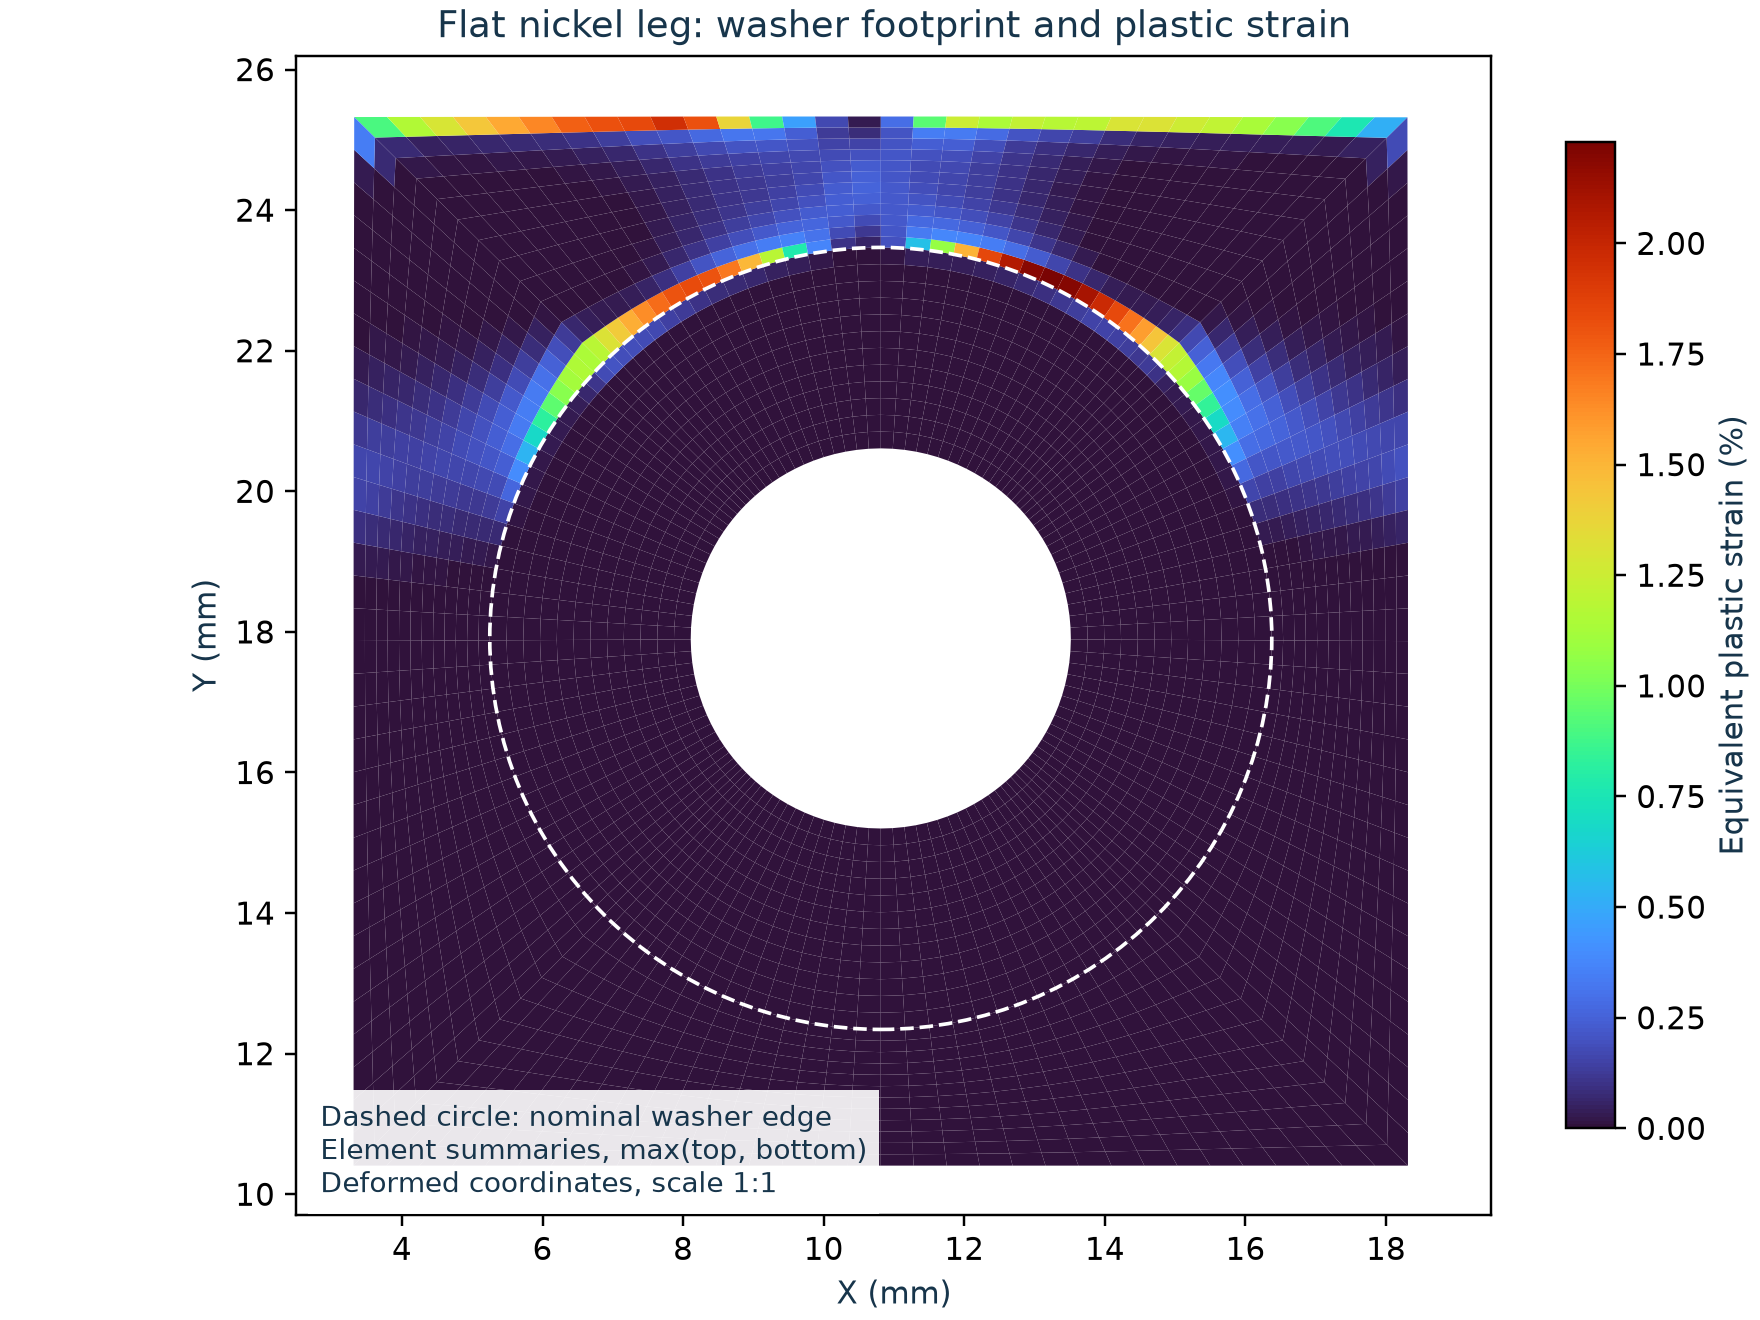
\includegraphics[width=.76\linewidth,height=102mm,keepaspectratio]{figures/friction_locked_fine_plastic_plan.png}
\captionof{figure}{Refined 750 N contact model at $u_X=+0.5$ mm. The lower nickel flat leg is shown in deformed coordinates at scale 1:1. Colour is the maximum of top/bottom shell element-summary plastic strain, not a fracture index.}\end{center}
\begin{center}\begin{tikzpicture}\begin{axis}[width=.98\linewidth,height=56mm,xlabel={Battery centre displacement (mm)},ylabel={Normal platen reaction (N)},xmin=0,xmax=.5,grid=both,legend style={font=\footnotesize,at={(.03,.97)},anchor=north west},xticklabel style={/pgf/number format/fixed,/pgf/number format/precision=2},tick label style={font=\small},label style={font=\small}]
\addplot+[color=Teal,thick,mark=none] table[col sep=comma,x=u,y=washer1] {data/friction_locked_clamp.csv};\addlegendentry{Coarse mesh}
\addplot+[color=Navy,thick,mark=none] table[col sep=comma,x=u,y=washer1] {data/friction_locked_fine_clamp.csv};\addlegendentry{Fine mesh}
\end{axis}\end{tikzpicture}

\captionof{figure}{Normal reaction at the first lower platen during the pull; the second platen gives essentially the same result. Both start at 750 N after the force-to-lock transfer. The fixed platen separation permits reaction to change under bending.}\end{center}
The refined contact calculation reports a maximum element-averaged penetration of 0.424 micrometres (0.283\% of strip thickness) over its saved history. The greatest accumulated plastic slip among the exported contact corner values is 1.071 micrometres. These contact quantities use a different sampling convention from the element-averaged sliding in the main table.\par
The pressure and sliding depend on the assumed friction coefficient, contact stiffness and rigid support idealization. Their numerical convergence and constitutive calibration are distinct questions. Small penetration is a numerical contact check; it does not establish that the real nickel, washer or PCB avoids indentation or tearing.
\clearpage\PageTitle{Verification and numerical limitations}
\ReportHeading{Mesh and rigid-battery coupling}
The shell mesh uses 2,304 elements in the coarse model and 9,216 in the refined model, with seven through-thickness integration points and full shell integration [3]. The maximum element edge-length ratio is approximately 3.02. Shared nodes connect each flat and vertical leg; attachment nodes and fixed clamp nodes are disjoint.

Production cases use Lagrange-multiplier MPC184 rigid beams at the battery interface [4]. Earlier direct-elimination attempts produced oscillatory corrections in frictional and refined cases. A coarse fixed-clamp comparison changed the endpoint force by only 0.0137\% when the rigid-coupling formulation was changed. This numerical comparison supports the replacement, but it is not experimental validation. Battery attachment footprint discretization changes slightly with the mesh and is part of the reported mesh sensitivity.

For fixed clamps, coarse-to-fine endpoint force changes by 5.18\% relative to the fine result, and the maximum difference across sampled curve points from 0.025 to 0.5 mm is 6.54\%. Peak plastic strain increases by 83.4\%. \textbf{The local strain is not mesh converged.} The force comparison is a sensitivity result, not a demonstrated asymptotic convergence rate.

For the contact model, refinement changes the endpoint reaction from 8.542 to 8.124 N (5.14\% relative to the fine value), while peak plastic strain changes from 1.254 to 2.228\%.

\ReportHeading{Acceptance and reaction checks}
Each accepted case completed its prescribed endpoint with no native solver errors. Native no-solve preflight checks verified element/node inventory before solving. Histories and final nodal/element tables are finite, time is monotone, and the target UX is reached.

An independent global force check sums all constrained reference/support reactions and applied preload. The acceptance limits are 1\% of $\max(|F_X|,1\ \mathrm{N})$ in X, 0.1 N in Y and 0.2 N in Z. These are numerical audit tolerances, not design allowables. The three contact cases additionally have global moment checks; translating the moment residual to the instantaneous battery centre gives a largest absolute component of 0.0201 N mm. Exact per-case residuals and warnings are retained in \texttt{ACCEPTED.json} and the native logs.

A postprocessing issue was corrected before accepting results: querying reaction at a free DOF can leave an APDL scalar unchanged. Reaction variables are now reset to zero before every query. Corrected read-only postprocessing was rerun from the saved database/result file; the physical solves were not changed.

\ReportHeading{Stopped attempts are not fracture observations}
Early frictional attempts and one refined direct-coupling attempt were stopped after oscillatory nonlinear corrections or excessive distortion. A two-step contact attempt also unintentionally ramped the newly imposed clamp displacement from zero; it was excluded and replaced by a separate force-to-lock transfer step. Their logs and results are retained for diagnosis. They are excluded from reported force curves. Solver nonconvergence is not evidence that the real strip broke. Production Lagrange-coupling runs are independently checked against their input hashes and equilibrium audit.

\ReportHeading{Warning review}
Lagrange-coupling cases can emit generic warnings about prescribed displacement on MPC nodes. The pull is applied at the common battery reference node; dependent attachment nodes are not independently constrained. Sparse-solver pivoting and a large-pivot-ratio warning are present in contact cases. A contact element also inherits the shell section number while using the friction material ID; the underlying structural shells retain material 1 (nickel), while contact material 2 supplies friction only. These warnings were reviewed against the input attributes and the reaction checks; conditioning remains a numerical limitation. Numerical completion does not resolve uncertainty in temper, geometry seating or joint attachment.

\clearpage\PageTitle{Reproducible procedure and next validation}
\ReportHeading{Reproduce the numerical result}
\begin{enumerate}
\item Extract the supplied source bundle into a writable local folder. Select a case with an \texttt{ACCEPTED.json} record. Each case includes its as-run \texttt{run.dat}, \texttt{preflight.dat}, mesh/configuration, corrected postprocessor, hashes and exported results.
\item Use ANSYS MAPDL 2026 R1.02 (26.1, UP20260202), N--mm--MPa units, sparse solver and shared-memory processing. Verify input SHA-256 hashes against the manifest. Use a fresh run folder and preserve the accepted one.
\item Run \texttt{preflight.dat} with one process and a pre/post license; it contains no \texttt{SOLVE}. Check zero errors and the inventory against \texttt{config.json}. Do not continue after a failed preflight.
\item Run \texttt{run.dat} with job name \texttt{pull}, four shared-memory threads and the structural license. The exact model, material law, supports and load steps are contained in this deck. Allow the solver to finish before extraction.
\item Run \texttt{post\_corrected.dat} with job name \texttt{post} in the same folder, using one process and a pre/post license (or the structural license if the pre/post seat is occupied). It reads \texttt{solved.db} and \texttt{pull.rst}; it does not solve. Check zero postprocessor errors.
\item Check the final load-step endpoint, finite histories, equilibrium limits and mesh table counts as described on the previous page. Compare force and strain with the bundled CSVs. Review warnings rather than relying only on the process exit code.
\item Compile this report with pdfLaTeX twice from its LaTeX folder. The PNGs remain external in \texttt{figures/}; the editable PGFPlots graphs read CSVs in \texttt{data/}. No raster data is encoded in the TeX source.
\end{enumerate}
Example native commands, run from the selected fresh case folder:
{\footnotesize\begin{verbatim}
ANSYS261.exe -b nolist -s noread -smp -np 1 -p preppost
             -j check -i preflight.dat -o preflight.out
ANSYS261.exe -b nolist -s noread -smp -np 4 -p ansys
             -j pull -i run.dat -o run.out
ANSYS261.exe -b nolist -s noread -smp -np 1 -p preppost
             -j post -i post_corrected.dat -o post_corrected.out
\end{verbatim}}
Each displayed two-line command is a single command when entered in a terminal. Read-only postprocessing also runs with \texttt{-p ansys}; that option was used when the Mechanical graphics session occupied the pre/post license. The reproduction bundle omits large binary result files; they are retained in the study workspace. Rerunning generates them from the supplied decks.

\ReportHeading{To obtain an actual snapping load}
Measure strip thickness, temper and formed radius, washer dimensions, weld footprint, real stack-up and retained bolt clamp force. Obtain a tensile curve from the same nickel stock, then test a washer/strip coupon and the assembled edge-battery joint under displacement control while recording force, displacement and failure location.

Replace the local washer region with a converged three-dimensional model; represent bolt/board compliance and weld failure if those paths matter. Calibrate fracture initiation and energy-based or characteristic-length-regularized evolution to the tests, and validate against an independent joint test. Extend the displacement ramp until a repeatable load drop and physical tear are reproduced. Report the force with uncertainty across material and joint variability, rather than declaring a strain maximum to be a break.

\clearpage\PageTitle{Sources and deliverables}
\ReportHeading{Primary references}
{\small
[1] Special Metals, \emph{Nickel 200}, technical bulletin. Tables 4 and 5 supply elastic constants and annealed-strip tensile ranges. Retrieved 5 October 2026. \href{https://www.specialmetals.com/documents/technical-bulletins/nickel-200.pdf}{Nickel 200 technical bulletin}.\par
[2] Special Metals, \emph{Nickel Alloy Handbook}, Nickel 200 typical annealed properties. Used only for the illustrative 148 MPa baseline yield stress. \href{https://www.specialmetals.com/documents/nickel-alloy-handbook.pdf}{Nickel Alloy Handbook}.\par
[3] ANSYS 2026 R1, \emph{SHELL181 Element Reference}. Shell formulation, integration and result storage. \href{https://ansyshelp.ansys.com/public/Views/Secured/corp/v261/en/ans_elem/Hlp_E_SHELL181.html}{SHELL181 documentation}.\par
[4] ANSYS 2026 R1, \emph{MPC184 Rigid Link/Beam}. Rigid coupling and direct-elimination/Lagrange-multiplier options. \href{https://ansyshelp.ansys.com/public/Views/Secured/corp/v261/en/ans_elem/Hlp_E_MPC184link.html}{MPC184 documentation}.\par
[5] ANSYS 2026 R1, \emph{CONTA174}, \emph{TARGE170}, and nonlinear static analysis guidance. \href{https://ansyshelp.ansys.com/public/Views/Secured/corp/v261/en/ans_elem/Hlp_E_CONTA174.html}{Contact element}; \href{https://ansyshelp.ansys.com/public/Views/Secured/corp/v261/en/ans_elem/Hlp_E_TARGE170.html}{target element}; \href{https://ansyshelp.ansys.com/public/Views/Secured/corp/v261/en/ans_str/Hlp_G_STR8_13.html}{nonlinear static analysis}.\par
[6] ANSYS 2026 R1, \emph{Material Reference: Damage Mechanics}. Calibration and damage-evolution framework for future fracture work; no damage model is used in this study. \href{https://ansyshelp.ansys.com/public/Views/Secured/corp/v261/en/ans_mat/mat_damageall.html}{Damage mechanics documentation}.\par
[7] ANSYS 2026 R1, \emph{Feature Archive / Material Reference}, bilinear isotropic hardening conventions. \href{https://ansyshelp.ansys.com/public/Views/Secured/corp/v261/en/pdf/ANSYS_Mechanical_APDL_Feature_Archive.pdf}{Feature Archive}; \href{https://ansyshelp.ansys.com/public/Views/Secured/corp/v261/en/pdf/ANSYS_Mechanical_APDL_Material_Reference.pdf}{Material Reference}.\par
}
\ReportHeading{Audit trail}
The study workspace is \texttt{outputs/battery\_side\_pull\_20261005} under the power-board project. It retains the CAD probe, material provenance, source hashes, attempted cases, accepted native logs and binary results. The source bundle contains the accepted cases, their CSV output and the report assets; it does not redistribute the manufacturer's full publications.

The original project is \texttt{powerboardsim\_v1.wbpj}. Geometry ID mappings and the numerical shell reconstruction are preserved in the audit and case configuration files. No accepted full-board modal or random-vibration result was replaced by this local study.

\ReportHeading{Accepted case directories}
{\small\begin{tabular}{l l}\toprule\textbf{Directory} & \textbf{Meaning}\\\midrule
\texttt{grip\_c1} & Direct-coupling diagnostic comparison \\
\texttt{grip\_lagrange} & Ideal clamp, +X, coarse \\
\texttt{grip\_fine\_lagrange} & Ideal clamp, +X, fine \\
\texttt{grip\_minus\_lagrange} & Ideal clamp, -X, coarse \\
\texttt{grip\_soft\_lagrange} & Ideal clamp, yield 105 MPa \\
\texttt{grip\_strong\_lagrange} & Ideal clamp, yield 210 MPa \\
\texttt{friction\_locked} & 750 N contact, +X, coarse \\
\texttt{friction\_locked\_minus} & 750 N contact, -X, coarse \\
\texttt{friction\_locked\_fine} & 750 N contact, +X, fine \\\bottomrule\end{tabular}}
\ReportHeading{Scope of the conclusion}
This is a reproducible computational investigation of local deformation and model sensitivity. It is not a qualification test, a validated fracture prediction, or evidence that the battery retention system is adequate. The missing material and joint calibration is a specific limitation that additional mesh density alone cannot remove.
\end{document}
